\section{RRT}

The \rrtfunnel\ algorithm will be based upon the general \ac{RRT}
algorithm\cite[LaValle]{article}. This means that it will be sampling based,
picking points uniformly from the state space, and expanding as quickly into the
state-space. An \ac{RRT} algorithm is inherently biased to grow towards
unexplored parts of the state space. A nice way of thinking about the \ac{RRT}
algorithm is as a \textit{Monte-Carlo} method that is biased towards the largest
\textit{Voronoi} region of a graph in the configuration space, as shown in
figure~\ref{subsec:voronoi regions}.

\subsection{The RRT algorithm}

The \ac{RRT} algorithm is a tree based algorithm which grows a tree in the
configuration space of the robot, starting with the root node at the base
configuration of the robot at hand. In order to expand the tree it draws a
sample at random from the configuration space, then tries to connect the new
sample with the nearest node in the tree. Nearest in the sense of some
predetermined distance metric. If a connection can be made -- meaning that it is
collision free, and satisfies the constraints of the dynamical model -- then a
new state is added to the tree. If the sampling is uniform, then the tree is
known to have the attribute that the probability of expanding from an existing
node in the tree is proportional the the \textit{Voronoi region} of that node,
and as the largest \textit{Voronoi regions} belongs to the states on the leaves
of the tree, this means that the tree will quickly expand into unexplored parts
of the state space, as can be seen in~(\ref{fig:rrt-expansion}),
and~(\ref{fig:rrt-voronoi})~\cite{Lav06}.

\begin{figure}
  \includegraphics{figures/rrt/rrt-pseudo.tex}
\end{figure}

\begin{figure}
  \centering
  \begin{minipage}[b]{0.3\textwidth}
    \includegraphics[width=\textwidth]{plainRRT10}
    \caption{RRT-tree after 10 iterations.}
  \end{minipage}
  \begin{minipage}[b]{0.3\textwidth}
    \includegraphics[width=\textwidth]{plainRRT50}
    \caption{RRT-tree after 50 iterations.}
  \end{minipage}
  \begin{minipage}[b]{0.3\textwidth}
    \includegraphics[width=\textwidth]{plainRRT100}
    \caption{RRT-tree after 100 iterations.}
  \end{minipage}
  \newline % Start the new line of plainRRT10.
  \begin{minipage}[b]{0.3\textwidth}
    \includegraphics[width=\textwidth]{plainRRT500}
    \caption{RRT-tree after 500 iterations.}
  \end{minipage}
  \begin{minipage}[b]{0.3\textwidth}
    \includegraphics[width=\textwidth]{plainRRT1000}
    \caption{RRT-tree after 1000 iterations.}
  \end{minipage}
  \begin{minipage}[b]{0.3\textwidth}
    \includegraphics[width=\textwidth]{plainRRT10000}
    \caption{RRT-tree after 10000 iterations.}
  \end{minipage}
  \caption{How the \ac{RRT} algorithm explores the state space.}
  \label{fig:rrt-expansion}
\end{figure}

Given a number of points in the plane, their Voronoi diagram divides the plane
according the the \textit{nearest neighbour rule}: Each point is associated with
the region of the plane closest to
it~\cite{aurenhammerVoronoiDiagramsSurvey1991}, as can be seen in the
figure~\ref{fig:voronoi-diagram}.

\begin{figure}
  \includegraphics[scale=.3]{figures/rrt/voronoi-diagram}
  \caption{Pictured: The Voronoi regions for a collection of points in the
    plane, using the standard Euclidean metric.}
  \label{fig:voronoi-diagram}
\end{figure}

When inspecting the Voronoi regions of a \ac{RRT} tree, it is apparent that the
leaf nodes will have the largest Voronoi regions, and thus also the largest
probability for getting expanded, as can be seen in
figure~\ref{fig:rrt-voronoi}.

\begin{figure}
  \frame{\includegraphics[clip, trim=5cm 9cm 5cm 9cm,
    scale=.5]{figures/rrt/rrtvoronoi}}
  \caption{Pictured: The voronoi regions for each node in a simple RRT tree,
    which shows how the voronoi bias will lead the algorithm towards unexplored
    areas quickly.}
  \label{fig:rrt-voronoi}
\end{figure}

The ability to quickly expand into the largest Voronoi regions of the
state-space is what enables the \ac{RRT} to avoid the \textit{curse of
  dimensionality} that is keeping other motion planning algorithms from being
employed on state-spaces of larger dimensionality. The expansion, and the
Voronoi regions, are dependent upon the metric function (\(\rho\)) used for
measuring distance in the state space. The optimal distance function would be
the optimal \textit{cost-to-go} function, which is the optimal cost to go from
one state to another on the optimal trajectory. However, solving the optimal
cost-to-go sub-problem for every node, is equivalent to solving the optimal
cost-to-go for the entire planning problem, and is thus not computationally
feasible~\cite{Lav06}. The cost-to-go can be any number of metrics such as the
energy consumed, time to target, or some distance metric in the state-space. For
differential constraints on the vehicle dynamics some metrics, such as the
Euclidean, may erode the performance of the algorithm, as it encorporates no
knowledge of the model's inability to move in certain directions, as
expamplified in~(\ref{fig:non-holonomic-vehicle-euclidean-weakness}). This is
not unexpected as the \textit{Euclidean metric} is only a proper metric for
holonomic vehicles \cite{parkFeedbackMotionPlanning2015}.

\begin{figure}
  \centering
  \includegraphics[scale=.2,angle=-90]{figures/rrtfunnel/non-holonomic-vehicle-euclidean-weakness}
  \caption{Consider two poses \(p_0\) and \(p_1\). Although \(p_1\) is nearer
    the robot in Euclidean distance it is harder to get to due to differential
    constraints. In this paper, we propose a directed distance function
    applicable to unicycle- type vehicles, that properly reflects the true
    cost-to-go of the system under the non-holonomic constraint. (figure
    courtesy of \cite{parkFeedbackMotionPlanning2015})}
  \label{fig:non-holonomic-vehicle-euclidean-weakness}
\end{figure}

\subsection{BiDirectional}

With a known end-goal in state-space it might be beneficial to start out at the
end-goal, and work backwards, towards the starting configuration, or growing a
tree from both, and then locally connect them once they meet.

\subsection{Dynamic RRT's?}

\begin{figure}
  \documentclass{standalone}
\usepackage{tikz}

\begin{document}
    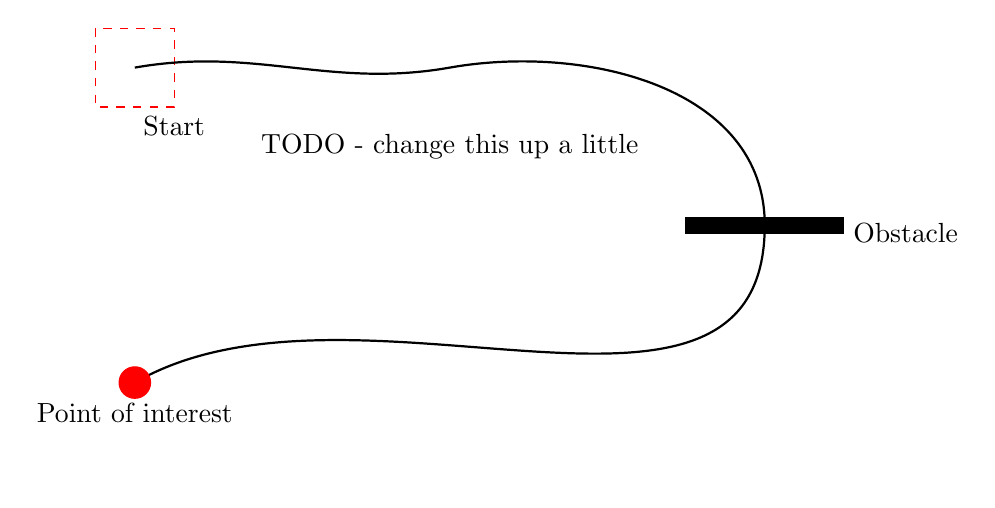
\begin{tikzpicture}
      \draw [red,dashed] (-2.5,2.5) rectangle (-1.5,1.5) node [black,below] {Start}; % Draws a rectangle
      \draw [thick] (-2,2) % Draws a line
      to [out=10,in=190] (2,2)
      to [out=10,in=90] (6,0) 
      to [out=-90,in=30] (-2,-2);    
      \draw [fill] (5,0.1) rectangle (7,-0.1) node [black,right] {Obstacle}; % Draws another rectangle
      \draw [red,fill] (-2,-2) circle [radius=0.2] node [black,below=4] {Point of interest}; % Draws a circle
      \draw node at (2,1) {TODO - change this up a little};
    \end{tikzpicture}
\end{document}
\end{figure}

\subsection{General framework under differential constraints} (LaValle p.676.)


\subsection{RDT}


\subsection{Dynamic RRT}

\subsection{Probabilistic completeness}

In general, even though the \ac{RRT} algorithm is sampling based, it will, as
time goes to infinity achieve probabilistic completeness in the state-space,
meaning that.

\subsection{Discrete RRT}

\subsection{RRT's with motion primitives}


\subsection{Motion Primitives}

A motion primitive is a discrete action chosen from some action set
\(\modelactionspace{}\), and applied as a constant action over a fixed period of
time. The time periods can vary in length, as the primitives do not need to have
the same time length. Thus in the model:
\[
  x_{k+1} = f_d(x_k,u_k)
\]
Where \(x_k = x((k-1)\delta{}t)\), and \(u_k\) is the action in
\(\modelactionspace{}_d\) that is applied from time \((k-1)\delta{}t\) to
\(k\delta{}t\). If we let \(\overline{u}^p\) be a motion primitive in
\(\modelactionspace{}\), which is a function from an interval of time, unto
\(modelactionspace{}\). Then by letting the interval of time start at 0 and stop
at \(t_F(\overline{u}^p)\), which has a final time that depends on the
particular prmitive~\cite{Lav06}.

The performance of the \ac{RRT} algorithm is dependent upon the control inputs
employed to search the state-space. For systems with few control inputs, random
control inputs can be sampled. The downside is that this usually produces
non-smooth motions. Instead, predefined motion primitives with with known
behaviour can be sampled, which will produce a smoother path, while also
reducing the complexity of the planning
task~\cite{vonasekGlobalMotionPlanning2013}. An example of this employed on a
humanoid robot can be found in~\cite{hauserUsingMotionPrimitives2008}. A simple
basis of motion primitives for a vehicle can therefore be 'turn-left',
'go-straight', or 'turn-right'. By chaining these basic smooth motion primitves
together a smooth path from the intial- to the goal-state can be found. A figure
displaying a tree built up from the tree motion primitives can be seen
in~(\ref{fig:motion-primitive-tree}).

\begin{figure}
  \centering
  \includegraphics[scale=.5]{figures/preliminaries/motion-primitive-tree}
  \caption{A simple motion primitive tree from the
    paper~\cite{vonasekHighlevelMotionPlanning2015}, displaying the composition
    of a left, right and a straight motion primitive.}
  \label{fig:motion-primitive-tree}
\end{figure}

Thus in essence robust motion primitives are beneficial as they seperate the
dynamics from the planner, enabling the planner to reason about what actions to
take, and not in what manner they should be executed.

\subsection{Funnel}

A Funnel is a motion primitive that is `guaranteed' to take the vehicle from a
set of initial conditions to a set of goal states.

\subsubsection{Composition of funnels}

In essence the Each funnel solves the subgoal of getting from the initial set of
the funnel to the goal set. Thus in essence each funnel solves the subproblem of
getting from one funnel to the next, and therefore composing funnels from some
global initial state to the goal state will have solve the motion planning
problem with the guarantees given by the tubes used for the planning task at
hand.

TODO - insert pretty picture of funnel with the integral curves of the extremal
paths embedded in beautiful red.

\subsubsection{Reachability plot for the Ground-Vehicle}
TODO - plot the reachability for the ground-vehicle in some time interval using
simulations.

TODO - plot A reachability tree in 3D using funnels - because different theta's
can exists at the same x,y positiions.

\subsection{Sampling}
It is important that the sampling sequence is dense in the space where sampling
occurs (state-space?), as we want resolution completeness in the end.
\subsubsection{How to obtain uniform sampling}
\subsubsection{How to define a good distance metric}
In general, it is not possible to get a perfect distance metric for our planning
problem, as this involves solving another optimal planning problem, and will
therefore be as, or more complex than the motion planning problem which is
already being solved. Therefore in general we will have to limit ourselves to
approximate distance metrics. The idea is to get as close to the optimal
cost-to-go function without having to compute expensive
computations~\cite{Lav06}. Distance metrics candidates in the RRT-Funnel
algorithm:
\begin{itemize}
\item Time - Since time can be found by simple summing up the time of all the
  funnels which need be added to get to the certain point in the configuration
  space.
\item Lyapunov function - As the Lyapunov function can be seen as an energy
  function, the cost to go to a point can (probably) be used as a metric in the
  planning.
\item Length of the shortest path between two configurations - ignoring
  collisions.
\item A* search heuristics.
\item Geometric - Stacking Funnels, where the shortest funnel of funnels wins.
  e.g. if the point is not in the cone projected out from the current state by
  the current motion primitives, pick the most extreme turn, and start over once
  again. If it can be reached by a turn, turn, then go straight for N-Funnels.
\end{itemize}

Note that most of these metrics are not metrics in the full sense, as they do
not fulfill the symmetric property, as under dynamic constraints going from a to
b, may not be the same as going from b to a. In most cases it is not true for a
nonholonomic vehicle.

\subsubsection{How to extend the tree?}

Should it be expanded into the dynamic Voronoi regions? If so, what are these
regions?


\subsection{Reachability Graph}

\subsection{RRT-Funnels}


\subsubsection{Transforming and composing the tubes}

If we look at the cyclic coordinates of our model, we can see that using `cyclic
coordinates', the dynamics is independent of position. Or rather:

\begin{math}
  \dot{\dot{q}} = \mathcal{L}(\dot{q},q)
\end{math}

TODO - finish this.


\subsubsection{Using Funnels as motion-primitives}

\subsubsection{Designing good motion primitives}
